\documentclass[fleqn,xcolor={usenames,dvipsnames}]{beamer}
\usepackage{amsmath} % {amssymb,amsfonts}
% \usepackage{colortbl}

% \usepackage{booktabs, multicol, multirow, adjustbox}
\usepackage{array, adjustbox,url}
\usepackage{pifont,marvosym} % wasysym

\usepackage{multimedia}
\usepackage[normalem]{ulem}
\usepackage{framed,color,ragged2e}
\usepackage[absolute,overlay]{textpos}
\definecolor{shadecolor}{rgb}{0.8,0.8,0.8}
\usetheme{boxes}
\setbeamertemplate{navigation symbols}{}
\usepackage{xcolor}
\usepackage{tikz}
\usetikzlibrary{shapes,arrows}
\usetikzlibrary{positioning}
\usetikzlibrary{calc}
% \usetikzlibrary{cd}
\usepackage[normalem]{ulem}

\newcolumntype{R}[2]{%
    >{\adjustbox{angle=#1,lap=\width-(#2)}\bgroup}%
    l%
    <{\egroup}%
}
\newcommand*\rot{\multicolumn{1}{R{45}{1em}}}% no optional argument here, please!


\title{Xolotl}
\subtitle{Compact mixnet format with hybrid anonymity
 and stronger forward secrecy}
% Now we have to build a GNU one!

\author[Burdges]{Jeff Burdges}
\institute{
  
\includegraphics[scale=0.2]{../logos/gnunet-logo.pdf}

  \vfill
  
\includegraphics[scale=0.2]{../logos/inria.pdf}
}
\date{28.6.2015}


\def\Z{\mathbb{Z}}


\begin{document}


{\setbeamertemplate{footline}{}
\begin{frame}
\titlepage
\end{frame}
}
\setcounter{framenumber}{0}


\begin{frame}{E-mail: Asynchronous messaging}
  \begin{itemize}
  \item Email with GnuPG provides authenticity and confidentiality... % \pause
  \item ... but fails to provide forward secrecy, aka key erasure,
  \item ... and fails to {\em protect meta-data}
  \end{itemize}  
\end{frame}


\begin{frame}{Ratchets provide forward-secrecy}
\begin{columns}[T]
\column{0.55\textwidth}
% Mexican walking fish
% salamander 
% gills resemble trees
% related to tiger salamander 
% neoteny metamorposis into similar salamander if given enough iodine or hormones 

Off-the-Record messaging: \\
\hspace*{2pt} Rerun DH key exchange occasionally 

\bigskip

Silence Circle's SCIMP: \\
\hspace*{2pt} Replace our key with its own hash \\
\hspace*{2pt} No sessions!

\bigskip

\onslide<2>{
Axolotl ratchet : \\
\hspace*{2pt} Weld these two together! 

% \bigskip 
% Used in Signal and WhatsApp
}

\column{0.45\textwidth}
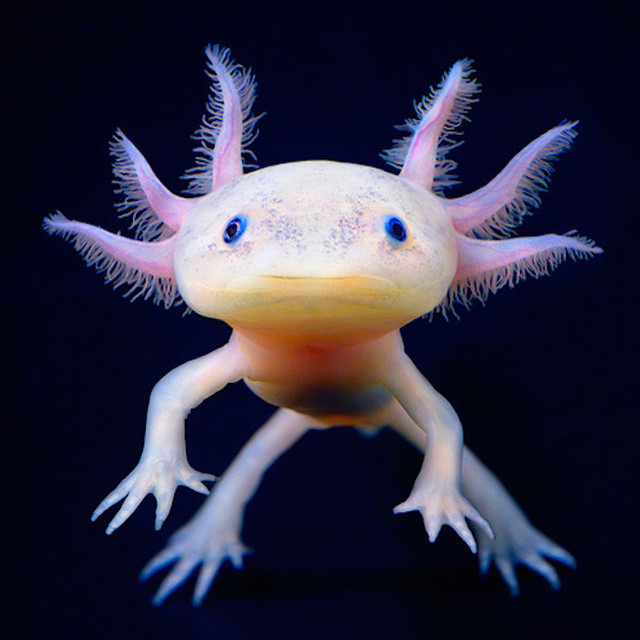
\includegraphics[width=\textwidth]{../pics/axolotl_animal-1.jpg}
\end{columns}

\medskip

\onslide<2>{
\begin{quote}
``[Axolotl] combines the .. forward secrecy [of] a hash iteration ratchet like SCIMP [with the] future secrecy .. of a DH ratchet like OtR'' % \\
\hfill --- Moxie Marlinspike % (TextSecure)
}
\end{quote}
\end{frame}


\begin{frame}{Axolotl ratchet by Trevor Perrin and Moxie Marlinspike}
\begin{columns}[T]
\column{0.6\textwidth}
Approach: \\
\hspace*{2pt} Run DH whenever possible \\
% \hspace*{5pt} 2-step vs 3-step \\
\hspace*{2pt} Iterate key by hashing otherwise 

\bigskip
2-step DH is less book keeping \\
\hspace*{2pt} than OtR's 3-step DH \\

\medskip
Header is one DH public key, \\
\hspace*{2pt} which one can encrypt.

\onslide<2>{
\bigskip
Neutral against Shor's algorithm \\
 \hspace*{2pt} running on a quantum computer. 
}

\column{0.4\textwidth}
\includegraphics[width=\textwidth]{../pics/axolotl_diagram}
% \vspace*{-20pt}
% \includegraphics[width=0.95\textwidth,trim={0 0 0 47},clip]{axolotl_diagram}
\end{columns}
\end{frame}


\begin{frame}{Axolotl questions}

Suggested questions on Axolotl during lunch, dinner, etc. : 

\medskip
\begin{itemize}
\item Just ``neutral'' against Shor's algorithm sounds weak.  \\ 
  Can one offer post-quantum forward-secrecy? \\ \medskip
\item How does one authenticate?  Is it deniable? \\ \medskip
\item I heard that punctured encryption adds key erasure to \\
  ordinary public key cryptography like GnuPG? \\
\end{itemize}

\end{frame}


% Metadata : entropique2015.tex

% Tor : ...

\begin{frame}[t]{Anonymity requires latency}
\begin{columns}[T]
\column{0.8\textwidth}
\hspace*{20pt} Can we just improve Tor?

\medskip

\hspace*{5pt} Tor is inherently vulnerable to correlation attacks \\
 \hspace*{10pt} {\em because} it must deliver many packets quickly.

\bigskip 

% Cryptography works, but 
\hspace*{5pt} Anonymity loves unrealistic ideals like

\column{0.2\textwidth}

\includegraphics[width=\textwidth]{../pics/tor/tor_onion}
% \vspace*{-20pt}
% \includegraphics[width=0.95\textwidth,trim={0 0 0 47},clip]{axolotl_diagram}
\end{columns}
\smallskip
\hspace*{1pt} ``All users are online all the time using constant bandwidth.''

\bigskip
\pause

\noindent We must therefore build applications to
\begin{itemize}
\item be tolerant to high latency, while still
\item being compelling to \sout{the anonymity set} users.
\end{itemize}

\smallskip

And we need an anonymizing transport that exploits this latency.

\end{frame}


\begin{frame}[t]{Onion Routing vs Mix Networks vs ...}

Academia's favored alternatives :
\begin{itemize}
\item Dining Cryptographers Networks (DC-nets) \\
 \hspace*{2pt} Aims for even lower latency. $O(n^2)$ bandwidth. 
\item Private Information Retrieval (PIR) \\
 \hspace*{2pt} Highly applications specific.  $O(n^2)$ bandwidth/computation
\item Verifiable mix networks \\
 \hspace*{2pt} Exposes packet dropping attacks. $O(n^2)$ computation
\end{itemize}

\end{frame}


\begin{frame}[t]{Onion Routing vs Mix Networks vs ...}

Anonymity tools need ``onion encryption'' and some routing, but..

\bigskip

Onion Routing means progressively establishing a fixed channel, \\
\hspace*{2pt} negotiating an ephemeral AKE with each hop. \\
\begin{itemize}
\item[Good] Stronger forward secrecy.  Inherently flexible.
\item[Bad] Easy correlation attacks.
\end{itemize}

\medskip

Mix networks encodes all routing and key material into one packet
\begin{itemize}
\item[Good] Better against correlation attacks.
\item[Bad] Relays cannot use ephemeral key material. 
\item[Mixed] Less flexible, facilitating analysis. \\
  New protocol :  No TCP, UDP, etc.
\end{itemize}

\end{frame}


\begin{frame}{Architecture}

Email handicapped past mix network efforts like Mixminion \\
 \hspace*{10pt} Do not attempt to support email!
\medskip

A mix network packet has a header, SURB, and body where
\begin{itemize}
\item the header is an onion of authenticated public-key exchanges,
\item the body is encrypted using a wide block cypher, \\
  but not authenticated, and
\item the Single-Use Reply Block (SURB) is a second header, \\
 \hspace*{2pt} providing recipient and two-way anonymity.
\end{itemize}
\[ \cdots \to S_{k-1} \to S_k \to \textrm{Cross} \to R_1 \to R_2 \to \cdots \]

\medskip
\pause

At a high level, our design constraints are to : 
\begin{itemize}
\item provide delivery properties using SURBs, and 
\item ensure users have the necessary SURBs.
\end{itemize}

\end{frame}


\begin{frame}[t]{Delivery strategy : Instant-ish }

\[ \begin{aligned}
\textrm{SURBs}\quad & \textrm{Rodger} \rightsquigarrow \textrm{Sam} \\
\textrm{Messages}\quad & \textrm{Sam} \to \cdots \to \textrm{Cross} \to \cdots \to R_k \to \textrm{Rodger}
\end{aligned} \]

Issues :
\begin{itemize}
\item Sam needs a {\em very recent} SURB from Rodger.  
\item $R_k$ should hold messages if Rodger went offline, but \\ 
 \hspace*{2pt} the Rodger's ``Guard'' $R_k$ knows their IP. \\
\end{itemize}

% \pause

Solutions : 
\begin{itemize}
\item Rodger asks Sam not to use his SURBs for long. \\
\item Rodger sends SURBs to $R_k$ when they connect later.
\end{itemize}

\bigskip
Are these measures sufficient?  No. \\
 \hspace*{2pt} Rodger might have too many guard nodes.

\end{frame}


\begin{frame}[t]{Delivery strategy : Checked mailbox}

\[ \begin{aligned}
\textrm{Long SURBs}\quad & \textrm{Rodger} \rightsquigarrow \textrm{Sam} \\
\textrm{Messages}\quad & \textrm{Sam} \to \cdots \to \textrm{Cross}
  \to \cdots \to R_k \to \textrm{Mailbox} \\
\textrm{Short SURBs}\quad & \textrm{Rodger} \to \cdots \to \textrm{Mailbox} \\
\textrm{Messages}\quad & \textrm{Mailbox} \to \cdots \to R_k \to \textrm{Rodger}
\end{aligned} \]

\smallskip

We win lovely delivery properties from the cross-over point 
 \hspace*{2pt} because Sam cannot flood, hack, etc. Rodger's mailbox server

\smallskip

Yet again :
\begin{itemize}
\item Sam needs a {\em less recent} and {\em longer lived} SURBs. % from Rodger.  
\item $R_k$ still holds messages if Rodger goes offline, but \\
 \hspace*{2pt} Rodger only provides it {\em short lived} SURBs.
\end{itemize}

% \pause

\medskip
Is this enough?  No.  \\
 \hspace*{2pt} No SURB can live forever!

\end{frame}


\begin{frame}[t]{Delivery strategy : Mailbox gateway}

\[ \begin{aligned}
\textrm{Credential}\quad & \textrm{Rodger} \rightsquigarrow \textrm{Sam} \\
\textrm{Long SURBs}\quad & \textrm{Rodger} \to \cdots \to \textrm{Gateway} \\
\textrm{Messages}\quad & \textrm{Sam} \to \cdots \to \textrm{Gateway} \\
\textrm{Messages}\quad & \textrm{Gateway} \to \cdots \to R_k \to \textrm{Mailbox} \\
 \cdots
\end{aligned} \]

% \smallskip

Credentials could be either 
\begin{itemize}
\item Single use HMAC tokens to limit Sam's message sending, 
\item VLR group signatures to let Sam send unlimited messages,
\item or nothing to allow a public contact point.
\end{itemize}

\bigskip
Is this one strategy to rule them all?  No. \\
 \hspace*{2pt} Sam can easily attack the gateway. \\
 \hspace*{2pt} And our instant-ish scheme is much faster.

\end{frame}


\begin{frame}{Sphinx by George Danezis and Ian Goldberg}

\begin{center}

\includegraphics[width=0.8\textwidth]{../pics/Sphinx}
% Mixnets use cryptography in mysterious ways

Sphinx is a packet format for an asynchronous mix network. 

\end{center}
\end{frame}


\begin{frame}{Sphinx by George Danezis and Ian Goldberg}
Sphinx is provably secure in the universal composability model \\
\hspace*{2pt} [Camenisch \& Lysyanskaya '05, Canetti '01]
\begin{enumerate}
\item Provides correct onion routing
\item Integrity, meaning immunity to long-path attacks
\item Security, including \\
\hspace*{2pt} wrap-resistance{\small $^*$} and \\
\hspace*{2pt} indistinguishability of forward and reply messages
\item[] Replay protection implemented by Bloom filter
\end{enumerate}

\bigskip

And Sphinx is far more compact than alternatives.

% Ask later about the caveats..

\bigskip

{\small $^*$ Wrap-resistance helps prevent nodes from acting as decryption oracles.}
\end{frame}


\begin{frame}{Sphinx by George Danezis and Ian Goldberg}
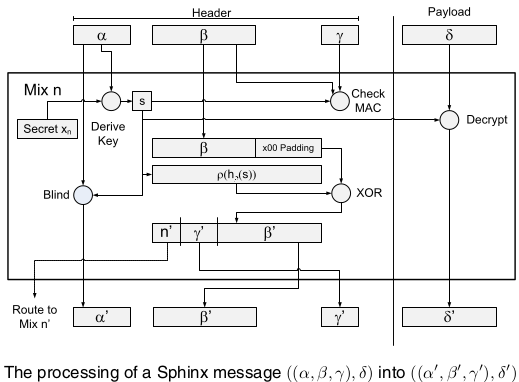
\includegraphics[width=\textwidth]{../pics/Sphinx-diagram}
\end{frame}
% LIONNESS???

\def\mathcomma{}

\begin{frame}{Build a Sphinx header}
First, select a sequence of $\nu$ nodes $n_i$ with keys $X_i = x_i G$ for $i<\nu$,
 an initial private scalar $a_0$, and
 the public curve point $\alpha_0 = a_0 G$.
Now recursively define 
\[ \begin{aligned}
\textrm{shared secret}\quad
 s_i &:= a_i X_i = x_i \alpha_i \mathcomma \\
\textrm{blinding factor}\quad
 b_i &:= H(\alpha_i,s_i) \mathcomma \\
\textrm{next private key}\quad
 a_{i+1} &:= b_i a_i \mathcomma \\ % \quad\textrm{and} \\
\textrm{next public key}\quad
 \alpha_{i+1} &:= b_i \alpha_i \quad\textrm{for $i < \nu$.} \\
\end{aligned} \]
% Our $i$th node replaces $\alpha_i$ by $\alpha_{i+1}$.

Next, compute the filler strings
\[ \begin{aligned}
 \phi_0 &:= \rho(\textrm{rnd})[0 \ldots z - \nu l] \\
 \phi_{i+1} &:= (\phi_i || 0_l) \oplus \rho(h_\rho(s_i))[ z-il \ldots z+l ] \\
\end{aligned} \]
where $l = |n| + |\gamma|$ and $l \nu < z = |\beta|$

\end{frame}


\begin{frame}{Build a Sphinx header}
Next, compute the filler strings
\[ \begin{aligned}
 \phi_0 &:= \Delta || \rho(\textrm{rnd})[0 \ldots z - \nu l - |\Delta|] \\
 \phi_{i+1} &:= (\phi_i || 0_l) \oplus \rho(H_\rho(s_i))[ z-il \ldots z+l ] \\
\end{aligned} \]
where $l = |n| + |\gamma|$ and $l \nu < z = |\beta|$

\medskip

Finally, generate the headers $M_i = (\alpha_i,\beta_i,\gamma_i)$ where 
\[ \begin{aligned}
 \beta_{\nu-1} &:= \big( 0_l \oplus \rho(H_\rho(s_{\nu-1}))[ 0 \ldots l ] \big)
   || \phi_{\nu-1} \\
 \beta_{i-1} &:= n_i || \gamma_i || \beta_i[0 \ldots z-l] \\
 \gamma_i &:= \textrm{HMAC}(s_i,\beta_i) \\
\end{aligned} \]

\medskip
Output $M_0$ and $s_0,\ldots,s_\nu$.

\end{frame}


\begin{frame}[t]{Replies vs. Key erasure}
Packet keys $a_0$ are ephemeral, but not node keys $x_i$.  

\medskip

Can nodes rotate keys?  \\
Yes, they do so for replay protection anyways, but..

\bigskip
\pause

Can a recipient be anonymous? \\
Yes!  With a Single-Use Reply Block (SURB).

\medskip
An anonymous recipient simply
\begin{itemize}
\item creates a Sphinx header $(\alpha, \beta, \gamma)$, 
 and a symmetric key $k$, 
\item communicates this to the sender $n$ in advance, and 
\item remembers these symmetric keys as each hop encrypts $\delta$.
\end{itemize}

\bigskip
\pause

Problem : SURB lifetime = Node key lifetime

\medskip
\hspace*{80pt} Can we do better?

\end{frame}


% delivery : 32c3.tex


% \begin{frame}{?}
% \end{frame}


\begin{frame}{Post-quantum Sphinx?}

A quantum computer factored 15 without cheating last year. \\
That might not sound like much progress for 20 years, but \\
\hspace*{3pt}  one should expect slow progress to continue, and \\
\hspace*{3pt}  one cannot expect negative results. \\

\medskip

We could worry for many decades even if they are impossible!

\end{frame}


\begin{frame}{Post-quantum Sphinx?}

We have two seemingly post-quantum key exchanges :
\begin{itemize}
\item Ring learning with errors and
\item Super-singular isogenies Diffie Hellman 
\end{itemize}

\medskip
In both cases, we need a blinding operations presumably based on
 the key exchange operation, but..
\begin{itemize}
\item anonymity is far more delicate than cryptography,
\item blinding is more fragile than key exchange, 
\item fewer researchers will ever study blinding, ..
\end{itemize}

\smallskip

And blinding is weakened by using multiple systems!

\end{frame}


\begin{frame}[t]{Ratchet for Sphinx}
\begin{columns}[T]
\column{0.60\textwidth}

Idea : Axolotl provides key erasure
\hspace*{5pt} and is neutral against Shor. % quantum computers.

\medskip

Can we integrate a ratchet with Sphinx?

\medskip
Axolotl won't work because : 
\begin{itemize}
\item Replays never message users
\item Cannot reuse curve elements
\end{itemize}

\medskip
Ideas : 
\begin{itemize}
\item Relays share new keys with the whole network for replay protection \\
% \hspace*{2pt} Key lifetime = SURB lifetime
\item Users should learn what messages made it eventually
\end{itemize}

\column{0.40\textwidth}

\includegraphics[width=1.35\textwidth,trim={80 0 0 0},clip]{../pics/Xolotl_muz}
\begin{center}
Xolotl \\
Sphinx + Axolotl
\end{center}
\end{columns}

\end{frame}


\begin{frame}[t]{Acknowledging ratchet state}
\begin{columns}[T]
\column{0.55\textwidth}
Idea: Client directs ratchet state

\bigskip
Chain keys evolve like Axolotl, 
 \hspace*{2pt} producing leaf keys. % \\ not message keys.

\smallskip
Create message keys by hashing \\
 \hspace*{2pt} a leaf key with a Sphinx ECDH \\ % result.
 \hspace*{10pt} $s_i := x_i \alpha_i$ \  ($= a_i X_i$) \\
\smallskip
 \hspace*{10pt} $\textrm{mk} := H(\textrm{lk},H'(s_i))$

\medskip
\onslide<2>{
Packets identify the message key from which their chain started.

\smallskip % \hspace*{2pt}
And their leaf key sequence no. % number.
%}

\smallskip
% \onslide<3>{ % \hspace*{2pt}
And parent max sequence no.
%And their parent chain's max sequence no.
}

\column{0.45\textwidth}
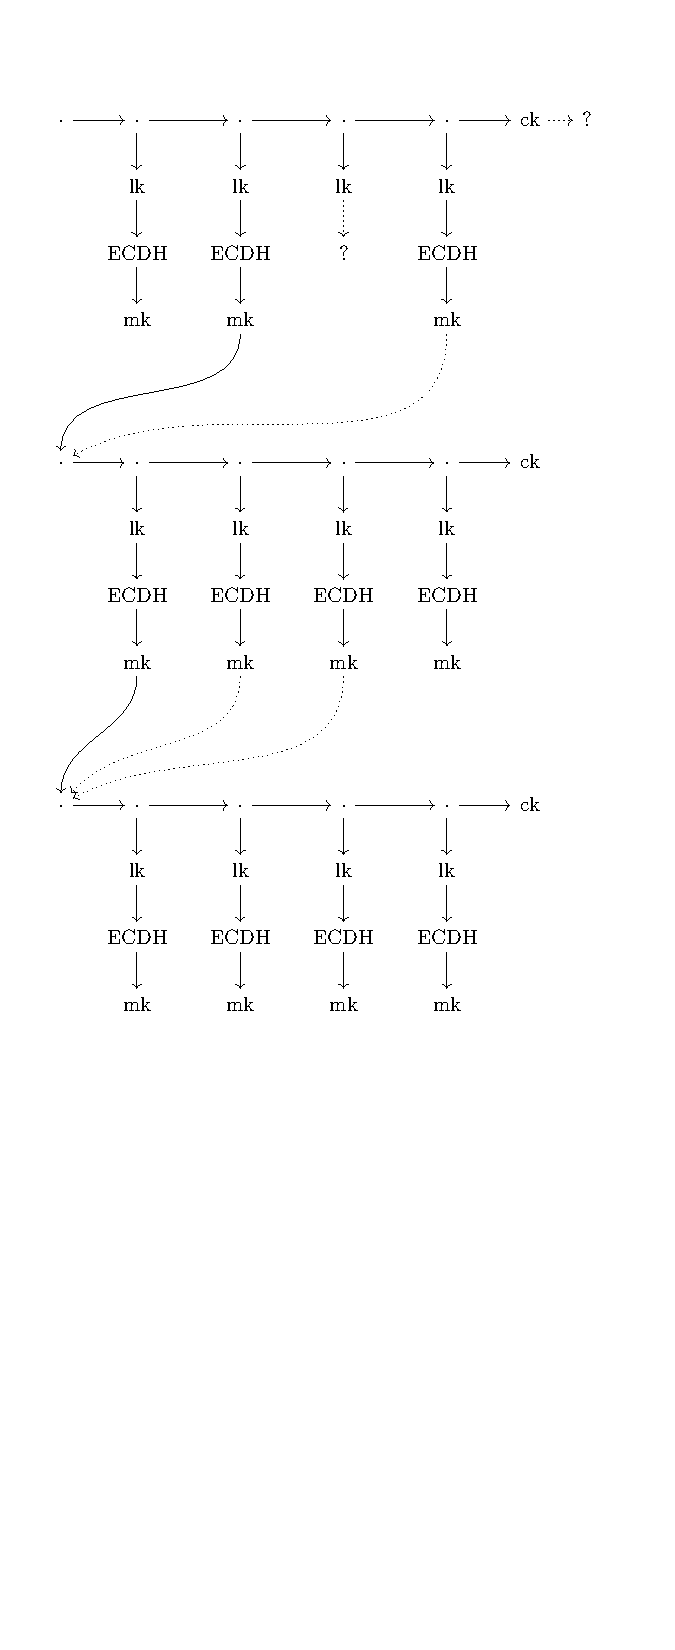
\includegraphics[width=\textwidth,trim={0 0 0 47},clip]{../up/32c3/Xolotl_diagram0}
\end{columns}
\end{frame}


\begin{frame}[t]{Tweaking Sphinx}
\begin{columns}[T]
\column{0.55\textwidth}

Not all hops need a ratchet, but \\
 \hspace*{1pt} ratchet hops must decrypt $\beta$ twice,
 \hspace*{1pt} requiring extra $\phi_j$. 

\medskip

We let $l$ differ for these virtual hops,
 \hspace*{1pt} so terms like $i l$ become $\sum_{j=0}^i l_j$.

\medskip

Ratchet hops replace $s_i$ by $\textrm{mk}$ \\
 \hspace*{1pt} in blinding $\alpha$ or decrypting $\delta$, while \\
 \hspace*{1pt} non-ratchet hops remain the same.

\column{0.45\textwidth}
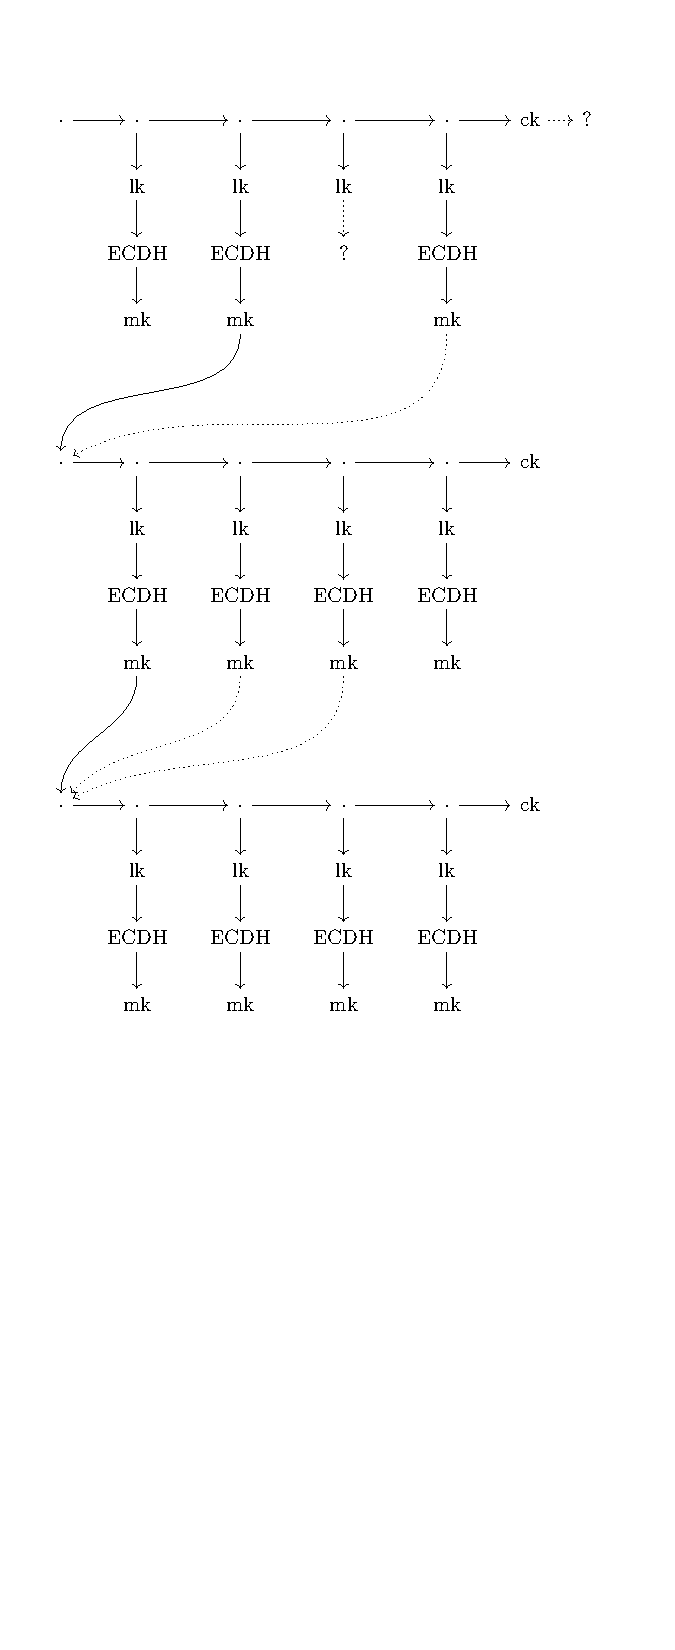
\includegraphics[width=\textwidth,trim={0 0 0 47},clip]{../up/32c3/Xolotl_diagram0}
\end{columns}
\end{frame}


\begin{frame}{Post-quantum?}
\begin{columns}[T]
\column{0.6\textwidth}
Ratchet hops improve key erasure, but..

\medskip

A quantum adversary can evolve all \\
 \hspace*{2pt} ratchets, including yours.

\medskip
\only<2>{
First, if ratchets live long enough, then \\
\hspace*{2pt} doing so might get expensive, \\
\hspace*{2pt} assuming ratchets names evolve.

\medskip

Second, we create new ratchets using \\
\hspace*{2pt} a post-quantum key exchange.

\smallskip

...}

\column{0.4\textwidth}

\includegraphics[width=1.2\textwidth]{../pics/Xolotl}
\end{columns}
\end{frame}


\begin{frame}{Aren't ratchet hops less anonymous?}

Isn't avoiding linking packets the whole point of Sphinx?

\medskip

A ratchet obviously links any two packets using it, \\
\hspace*{2pt} but that's no where near the end of the story.

\bigskip

First, we can judiciously intermix ratchet and non-ratchet hops.
\[ \textrm{User} \to \textrm{Guard} \to \textrm{Normal} \to \textrm{Ratchet} \to \textrm{Normal} \to \textrm{Cross} \to \cdots \]

\smallskip
Second, ratchets need not always be owned by the same user!

\end{frame}



\end{document}










\begin{frame}{Xolotl questions}

Suggested questions on Axolotl during lunch, dinner, etc. : 

\medskip
\begin{itemize}
\item What post \\ \medskip
\item  \\ \medskip
\item Is it safe to use a ratchet given to you by a friend?  \\
\end{itemize}

\end{frame}









\begin{frame}[t]{Relay key replacement }
Replay protection requires that relays replace keys regularly. 
\begin{columns}[T]
\column{0.6\textwidth}
{\hfil Replay key lifetime = SURB lifetime \hfil}

\medskip
Longer lifetime improves:
\begin{itemize}
\item Delivery convenience
\end{itemize}

\smallskip
Shorter lifetime improves:
\begin{itemize}
\item Throughput 
\item Memory footprint
\item Forward-secrecy
\end{itemize}

\column{0.4\textwidth}

\includegraphics[width=1.2\textwidth]{../pics/Xolotl}
\end{columns}
\end{frame}







\pause\medskip
I doubted that SIDH admired the blinding used in Sphinx, \\
\hspace*{3pt} but recently my opinion has changed. \\

\smallskip

% There are nevertheless several disadvantages, like
% \begin{itemize}
% \item 0.5kb+ public keys, and
% \item 300 times slower than curve25519!
% \end{itemize}

We'd need composing isogenies to give a blinding operation too. 

\smallskip

And SIDH is 300 times slower than curve25519 anyways!










\begin{frame}{A Ring-LWE straw-man Sphinx}

We have a ring $R = (\Z/p\Z)[x]/\Phi(x)$ where ... \\
\hspace*{3pt} $\Phi(x)$ is irreducible of degree 1024, maybe cyclotomic,
 and $p>1024$ is prime. 
\smallskip

A private key is polynomials $s$ and $e$ with small coefficients, \\
\hspace*{3pt} while a public key is a random $a\in R$ and $b = s a + e$.

\pause\smallskip
A candidate blinding operation might be, pick $s'$, $e'$, and $e''$ small, \\
\hspace*{3pt} to compute $a' = s' a + e'$ and $b' = s' b + e''$.

\smallskip
Imagine a path $n_1 \to n_2 \to n_3$ where $n_2$ is honest but \\
\hspace*{3pt}  $n_1$ and $n_3$ controlled by the adversary.
\begin{align*}
a' b &= (s' a + e') (s a + e) = s' s a^2 + s' a e + e' s a + e' e \\
a b' &= (s' (s a + e) + e'')a = s' s a^2 + s' e a + e'' a \\
a' b - a b' &= e' s a + e' e - e'' a
= e' b - e'' a
= (e' s - e'') a + e' e
\end{align*}

\end{frame}





